\documentclass[a3paper,landscape]{article}
\usepackage[margin=0.7in]{geometry}

\usepackage{tikz}
\usetikzlibrary{arrows,positioning,shapes.geometric,calc, shapes, shapes.gates.logic.US}
\title{Network Threats Taxonomy}

%%%%%%%%%%%%%%%%%%%%% Variables %%%%%%%%%%%%%%%%%%%%%
%%%%%%%%%%% Displacements %%%%%%%%%%%
\def \southXDisplacement {1}
\def \southBorderXDisplacement {1.3}

%%%%%%%%%%% Distances %%%%%%%%%%%
\def \headerNodeDistance {2.5cm}
\def \halfHeaderNodeDistance {\headerNodeDistance / 2}
\def \largeY {1.2cm}
\def \medY {0.5cm}
\def \smallY {0.2cm}
\def \shiftX {-2cm}

\tikzset{
 	headerblock/.style= {draw=none, rectangle, align=center,minimum width=2.5cm,minimum height=0.75cm, fill=gray!30, font=\bf}, 
 	block/.style= {draw, rectangle, align=center,minimum width=2.4cm,minimum height=0.5cm, font=\bfseries}, 
 	roundedblock/.style= {draw, ellipse, align=center, font=\bfseries, inner sep=0.06cm}, 
 	semiroundedblock/.style= {draw, rounded rectangle, rounded rectangle west arc=0pt, align=center, font=\bfseries, minimum width=2.4cm, minimum height=0.75cm}, 
	sectionblock/.style= {draw, rectangle, rounded corners=1em, align=center,minimum width=38cm,minimum height=0.75cm, fill=gray!15, font=\bf}
 }
 
 
\begin{document}

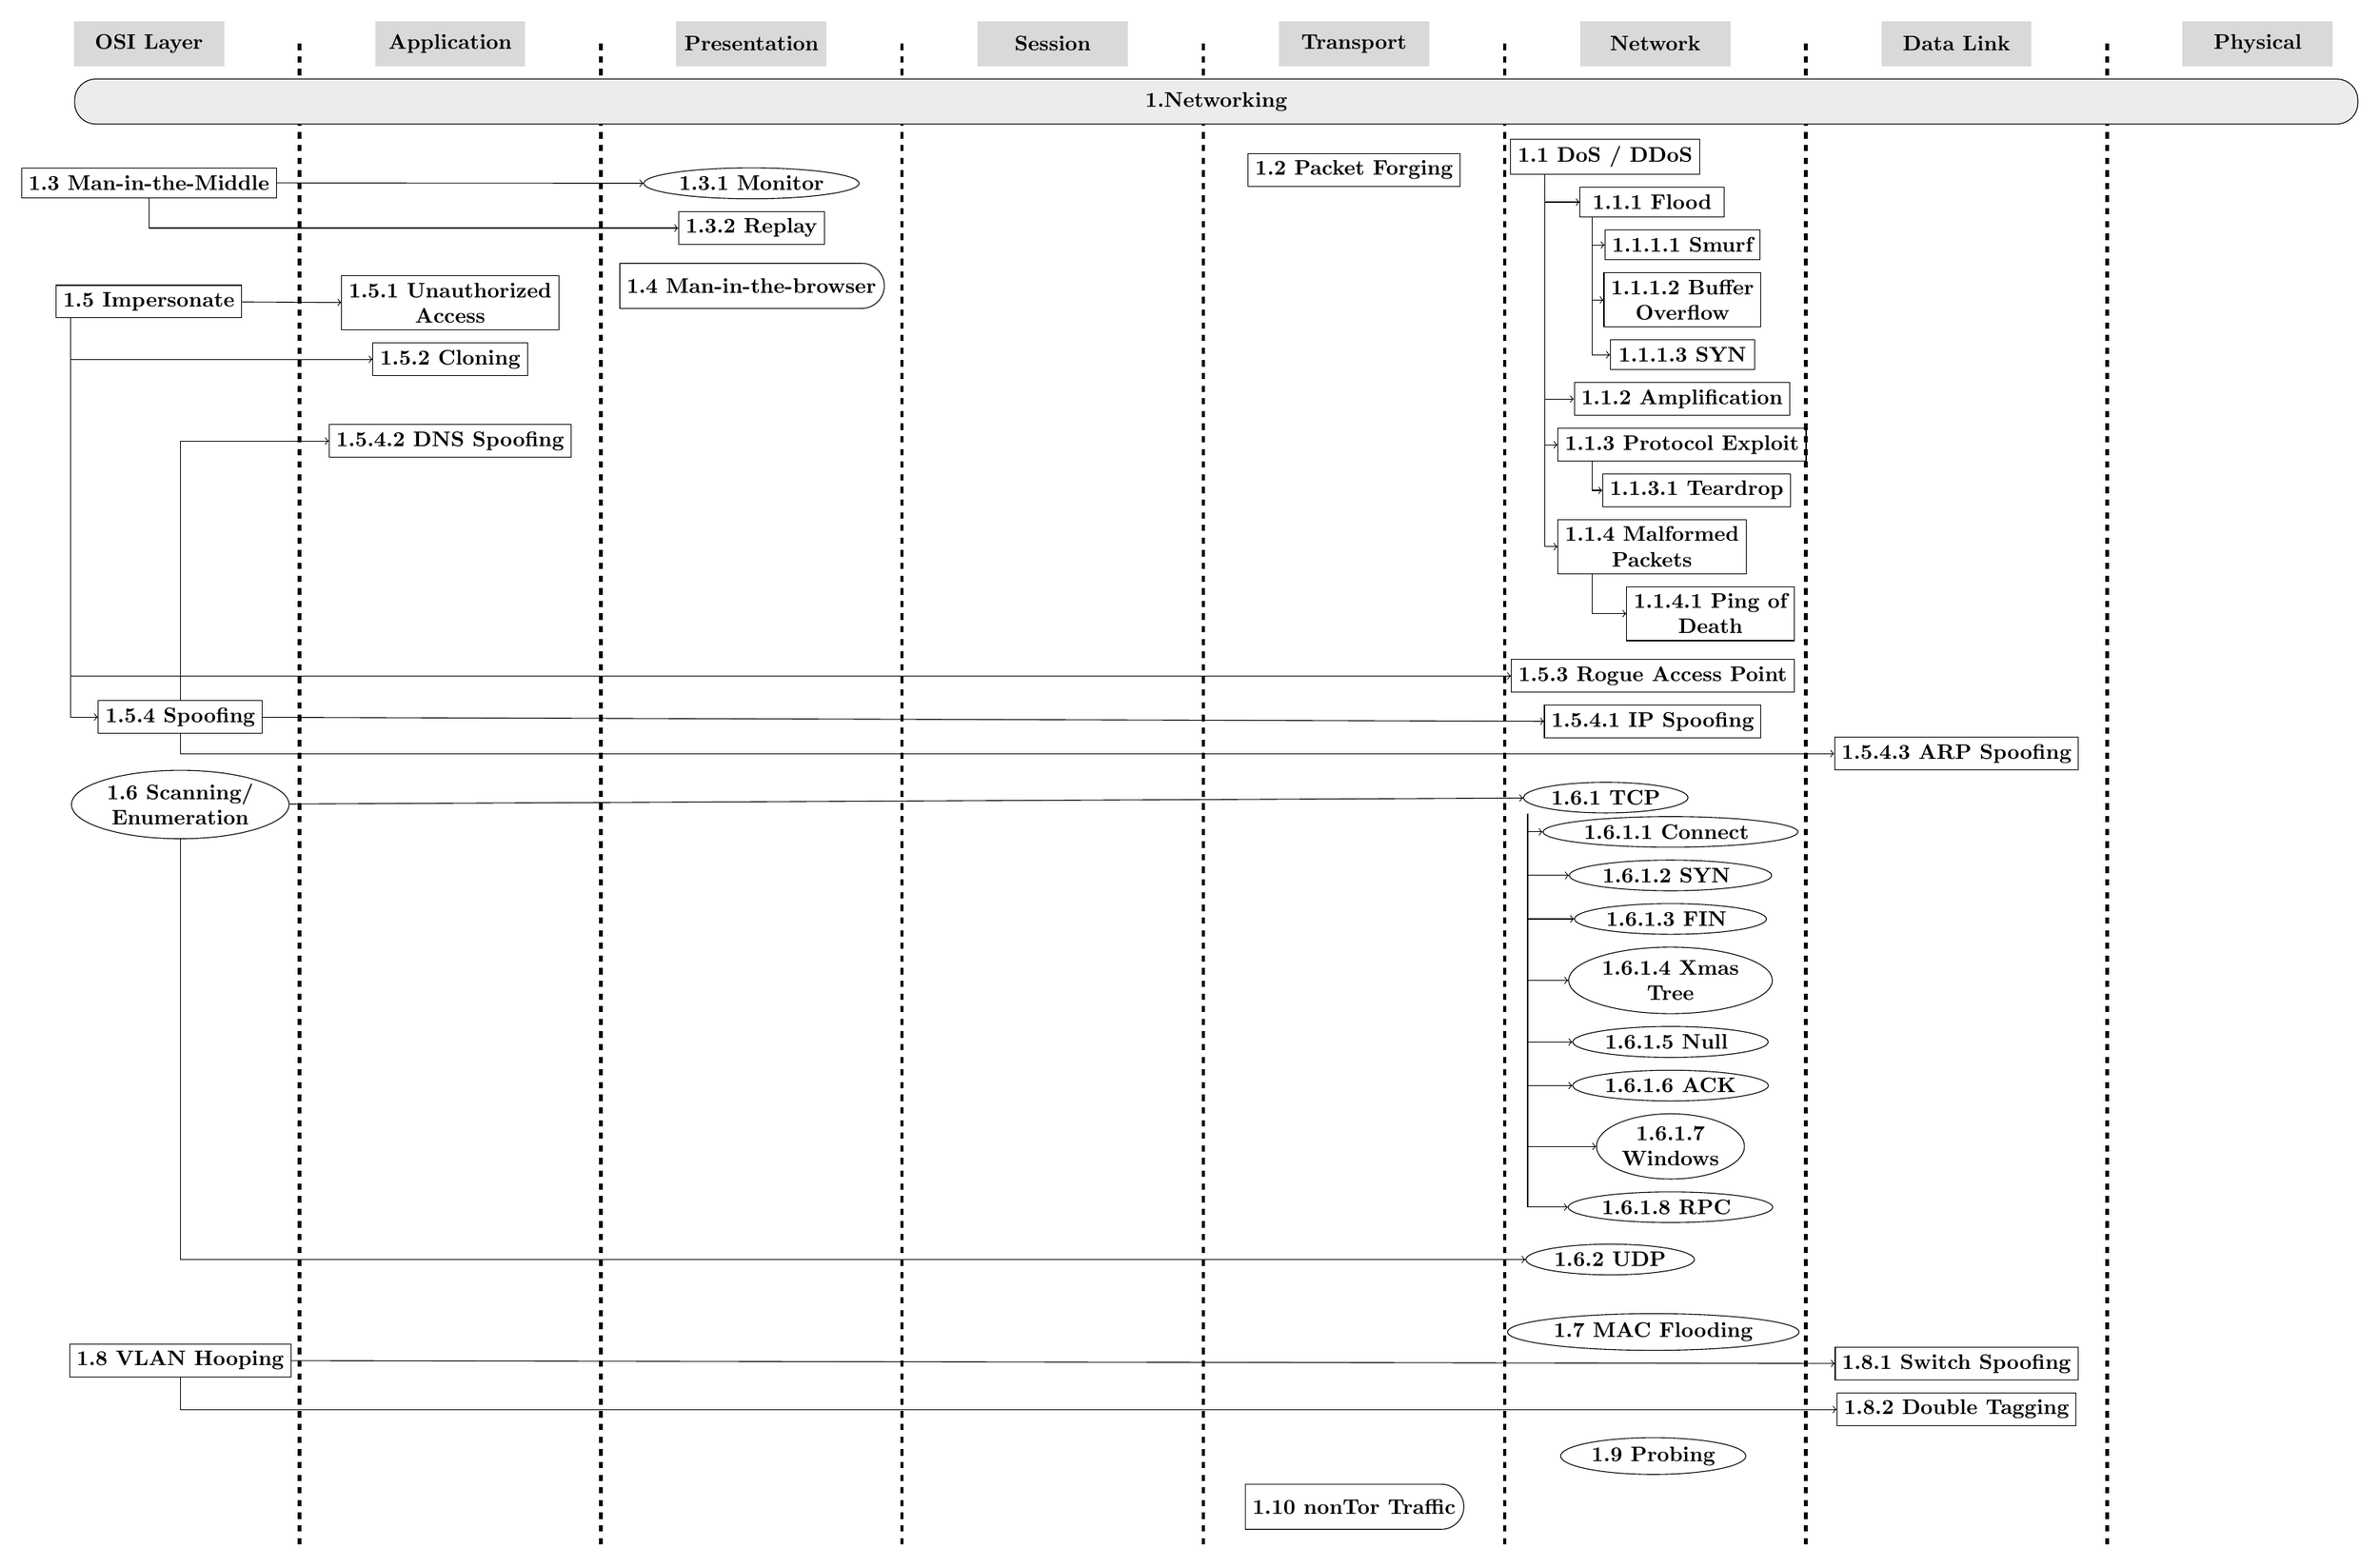
\begin{tikzpicture}
	
    \node [headerblock] (None) {OSI Layer};
\node [headerblock, right =\headerNodeDistance of None] (A) {Application};
\node [headerblock, right =\headerNodeDistance of A] (P) {Presentation};
\node [headerblock, right =\headerNodeDistance  of P] (S) {Session};
\node [headerblock, right =\headerNodeDistance  of S] (T) {Transport};
\node [headerblock, right =\headerNodeDistance  of T] (N) {Network};
\node [headerblock, right =\headerNodeDistance  of N] (D) {Data Link};
\node [headerblock, right =\headerNodeDistance  of D] (H) {Physical};
    \draw [dashed, ultra thick] ($(None.east)+(\halfHeaderNodeDistance,0)$) -- ($(None.east)+(\halfHeaderNodeDistance,-25)$);
\draw [dashed, ultra thick] ($(A.east)+(\halfHeaderNodeDistance,0)$) -- ($(A.east)+(\halfHeaderNodeDistance,-25)$);
\draw [dashed, ultra thick] ($(P.east)+(\halfHeaderNodeDistance ,0)$) -- ($(P.east)+(\halfHeaderNodeDistance ,-25)$);
\draw [dashed, ultra thick] ($(S.east)+(\halfHeaderNodeDistance ,0)$) -- ($(S.east)+(\halfHeaderNodeDistance ,-25)$);
\draw [dashed, ultra thick] ($(T.east)+(\halfHeaderNodeDistance ,0)$) -- ($(T.east)+(\halfHeaderNodeDistance,-25)$);
\draw [dashed, ultra thick] ($(N.east)+(\halfHeaderNodeDistance ,0)$) -- ($(N.east)+(\halfHeaderNodeDistance,-25)$);
\draw [dashed, ultra thick] ($(D.east)+(\halfHeaderNodeDistance ,0)$) -- ($(D.east)+(\halfHeaderNodeDistance,-25)$);

%%%%%%%%%%%%%%%%%%%%% Nodes %%%%%%%%%%%%%%%%%%%%%
	\node [sectionblock, below right =\smallY and -\headerNodeDistance of None] (S1) {1.Networking};
    
    \node [block, below left=\largeY and \shiftX of N] (1_1) {1.1 DoS / DDoS};
	\node [block, below right=\smallY and \shiftX of 1_1] (1_1_1) {1.1.1 Flood};
    \node [block, below right=\smallY and \shiftX of 1_1_1] (1_1_1_1) {1.1.1.1 Smurf};
    \node [block, below =\smallY of 1_1_1_1] (1_1_1_2) {1.1.1.2 Buffer\\Overflow};
    \node [block, below =\smallY of 1_1_1_2] (1_1_1_3) {1.1.1.3 SYN};
    \node [block, below left=\smallY and \shiftX*1.5 of 1_1_1_3] (1_1_2) {1.1.2 Amplification};
    \node [block, below =\smallY of 1_1_2] (1_1_3) {1.1.3 Protocol Exploit};
    \node [block, below right=\smallY and \shiftX*1.7 of 1_1_3] (1_1_3_1) {1.1.3.1 Teardrop};
    \node [block, below left=\smallY and \shiftX*1.2 of 1_1_3_1] (1_1_4) {1.1.4 Malformed\\Packets};
    \node [block, below right=\smallY and \shiftX of 1_1_4] (1_1_4_1) {1.1.4.1 Ping of\\Death};

   	\node [block, below =\largeY*1.2 of T] (1_2) {1.2 Packet Forging};

	\node [block, below =\largeY*1.4 of None] (1_3) {1.3 Man-in-the-Middle};
	\node [roundedblock, below =\largeY*1.4 of P] (1_3_1) {1.3.1 Monitor};
    \node [block, below =\smallY of 1_3_1] (1_3_2) {1.3.2 Replay};
    
	\node [semiroundedblock, below =\smallY*1.5 of 1_3_2] (1_4) {1.4 Man-in-the-browser};

	\node [block, below =\largeY*1.2 of 1_3] (1_5) {1.5 Impersonate};
	\node [block, below =\largeY*2.9 of A] (1_5_1) {1.5.1 Unauthorized\\Access};
    \node [block, below =\smallY of 1_5_1] (1_5_2) {1.5.2 Cloning};
    \node [block, below left =\smallY*1.5 and \shiftX*1.4 of 1_1_4_1] (1_5_3) {1.5.3 Rogue Access Point};
    \node [block, below right =\largeY*5.3 and \shiftX*1.2 of 1_5] (1_5_4) {1.5.4 Spoofing};
    \node [block, below =\smallY of 1_5_3] (1_5_4_1) {1.5.4.1 IP Spoofing};
    \node [block, below =\smallY*4 of 1_5_2] (1_5_4_2) {1.5.4.2 DNS Spoofing};
    \node [block, below =\largeY*9.3 of D] (1_5_4_3) {1.5.4.3 ARP Spoofing};
    
    \node [roundedblock, below =\smallY*3 of 1_5_4] (1_6) {1.6 Scanning/\\Enumeration};
    \node [roundedblock, below left=\largeY/1.5 and \shiftX of 1_5_4_1] (1_6_1) {1.6.1 TCP};
	\node [roundedblock, below right=\smallY and \shiftX*0.7 of 1_6_1] (1_6_1_1) {1.6.1.1 Connect };
	\node [roundedblock, below =\smallY of 1_6_1_1] (1_6_1_2) {1.6.1.2 SYN };
	\node [roundedblock, below =\smallY of 1_6_1_2] (1_6_1_3) {1.6.1.3 FIN };
	\node [roundedblock, below =\smallY of 1_6_1_3] (1_6_1_4) {1.6.1.4 Xmas\\Tree};
	\node [roundedblock, below =\smallY of 1_6_1_4] (1_6_1_5) {1.6.1.5 Null };
	\node [roundedblock, below =\smallY of 1_6_1_5] (1_6_1_6) {1.6.1.6 ACK};
    \node [roundedblock, below =\smallY of 1_6_1_6] (1_6_1_7) {1.6.1.7\\Windows };
	\node [roundedblock, below =\smallY of 1_6_1_7] (1_6_1_8) {1.6.1.8 RPC };
	\node [roundedblock, below left =\medY and \shiftX*0.6 of 1_6_1_8] (1_6_2) {1.6.2 UDP};
	
    \node [roundedblock, below right =\smallY*4 and \shiftX of 1_6_2] (1_7) {1.7 MAC Flooding};

    \node [block, below =\largeY*7 of 1_6] (1_8) {1.8 VLAN Hooping};
    \node [block, below =\largeY*8 of 1_5_4_3] (1_8_1) {1.8.1 Switch Spoofing};
    \node [block, below =\smallY of 1_8_1] (1_8_2) {1.8.2 Double Tagging};
	
    \node [roundedblock, below =\largeY*1.2 of 1_7] (1_9) {1.9 Probing};
    \node [semiroundedblock, below =\largeY*18 of 1_2] (1_10) {1.10 nonTor Traffic};

%%%%%%%%%%%%%%%%%%%%% Links %%%%%%%%%%%%%%%%%%%%%
	\draw[->] ($(1_1.south)-(\southXDisplacement, 0)$) |- (1_1_1.west) ;
    \draw[->] ($(1_1_1.south)-(\southXDisplacement, 0)$) |- (1_1_1_1.west) ;
    \draw[->] ($(1_1_1.south)-(\southXDisplacement, 0)$) |- (1_1_1_2.west) ;
    \draw[->] ($(1_1_1.south)-(\southXDisplacement, 0)$) |- (1_1_1_3.west) ;
   	\draw[->] ($(1_1.south)-(\southXDisplacement, 0)$) |- (1_1_2.west) ;
    \draw[->] ($(1_1.south)-(\southXDisplacement, 0)$) |- (1_1_3.west) ;
    \draw[->] ($(1_1_3.south)-(\southXDisplacement*1.5, 0)$) |- (1_1_3_1.west) ;
    \draw[->] ($(1_1.south)-(\southXDisplacement, 0)$) |- (1_1_4.west) ;
    \draw[->] ($(1_1_4.south)-(\southXDisplacement, 0)$) |- (1_1_4_1.west) ;
    \draw[->] (1_3) -- (1_3_1);
    \draw[->] (1_3) |- (1_3_2);
	\draw[->] (1_5) -- (1_5_1);
    \draw[->] ($(1_5.south)-(\southBorderXDisplacement, 0)$) |- (1_5_2.west) ;
	\draw[->] ($(1_5.south)-(\southBorderXDisplacement, 0)$) |- (1_5_3.west) ;
	\draw[->] ($(1_5.south)-(\southBorderXDisplacement, 0)$) |- (1_5_4.west) ;
	\draw[->] (1_5_4) -- (1_5_4_1);
	\draw[->] ($(1_5_4.north)$) |- (1_5_4_2.west) ;
	\draw[->] ($(1_5_4.south)$) |- (1_5_4_3.west) ;
	\draw[->] (1_6) -- (1_6_1);
	\draw[->] ($(1_6_1.south)-(\southBorderXDisplacement, 0)$) |- (1_6_1_1.west) ;
	\draw[->] ($(1_6_1.south)-(\southBorderXDisplacement, 0)$) |- (1_6_1_2.west) ;
	\draw[->] ($(1_6_1.south)-(\southBorderXDisplacement, 0)$) |- (1_6_1_3.west) ;
	\draw[->] ($(1_6_1.south)-(\southBorderXDisplacement, 0)$) |- (1_6_1_4.west) ;
	\draw[->] ($(1_6_1.south)-(\southBorderXDisplacement, 0)$) |- (1_6_1_5.west) ;
	\draw[->] ($(1_6_1.south)-(\southBorderXDisplacement, 0)$) |- (1_6_1_6.west) ;
	\draw[->] ($(1_6_1.south)-(\southBorderXDisplacement, 0)$) |- (1_6_1_7.west) ;
	\draw[->] ($(1_6_1.south)-(\southBorderXDisplacement, 0)$) |- (1_6_1_8.west) ;
	\draw[->] ($(1_6.south)$) |- (1_6_2.west) ;
	\draw[->] (1_8) -- (1_8_1);
  	\draw[->] ($(1_8.south)$) |- (1_8_2.west) ;
    
\end{tikzpicture}
\begin{tikzpicture}
	
    \node [headerblock] (None) {OSI Layer};
\node [headerblock, right =\headerNodeDistance of None] (A) {Application};
\node [headerblock, right =\headerNodeDistance of A] (P) {Presentation};
\node [headerblock, right =\headerNodeDistance  of P] (S) {Session};
\node [headerblock, right =\headerNodeDistance  of S] (T) {Transport};
\node [headerblock, right =\headerNodeDistance  of T] (N) {Network};
\node [headerblock, right =\headerNodeDistance  of N] (D) {Data Link};
\node [headerblock, right =\headerNodeDistance  of D] (H) {Physical};
    \draw [dashed, ultra thick] ($(None.east)+(\halfHeaderNodeDistance,0)$) -- ($(None.east)+(\halfHeaderNodeDistance,-25)$);
\draw [dashed, ultra thick] ($(A.east)+(\halfHeaderNodeDistance,0)$) -- ($(A.east)+(\halfHeaderNodeDistance,-25)$);
\draw [dashed, ultra thick] ($(P.east)+(\halfHeaderNodeDistance ,0)$) -- ($(P.east)+(\halfHeaderNodeDistance ,-25)$);
\draw [dashed, ultra thick] ($(S.east)+(\halfHeaderNodeDistance ,0)$) -- ($(S.east)+(\halfHeaderNodeDistance ,-25)$);
\draw [dashed, ultra thick] ($(T.east)+(\halfHeaderNodeDistance ,0)$) -- ($(T.east)+(\halfHeaderNodeDistance,-25)$);
\draw [dashed, ultra thick] ($(N.east)+(\halfHeaderNodeDistance ,0)$) -- ($(N.east)+(\halfHeaderNodeDistance,-25)$);
\draw [dashed, ultra thick] ($(D.east)+(\halfHeaderNodeDistance ,0)$) -- ($(D.east)+(\halfHeaderNodeDistance,-25)$);

%%%%%%%%%%%%%%%%%%%%% Nodes %%%%%%%%%%%%%%%%%%%%%
	\node [sectionblock, below right =\smallY and -\headerNodeDistance of TCP] (S2) {2. Host};
	
    \node [block, below = \largeY of TCP] (2_1) {2.1 Malware};
    \node [block, below left=\largeY*1.8 and \shiftX of A] (2_1_1) {2.1.1 Trojans};
	\node [block, below right=\smallY and \shiftX*0.8 of 2_1_1] (2_1_1_1) {2.1.1.1 Remote\\Access};
	\node [block, below =\smallY of 2_1_1_1] (2_1_1_2) {2.1.1.2 Sending};
	\node [block, below =\smallY of 2_1_1_2] (2_1_1_3) {2.1.1.3 Destructive};
	\node [block, below =\smallY of 2_1_1_3] (2_1_1_4) {2.1.1.4 Proxy};
	\node [block, below =\smallY of 2_1_1_4] (2_1_1_5) {2.1.1.5 FTP};
	\node [block, below =\smallY of 2_1_1_5] (2_1_1_6) {2.1.1.6 Security\\Software Disable};
	\node [block, below =\smallY of 2_1_1_6] (2_1_1_7) {2.1.1.7 DoS};
    
	\node [block, below left =\medY*0.5 and \shiftX*0.8 of 2_1_1_7] (2_1_2) {2.1.2 Worm};
    
	\node [block, below =\smallY of 2_1_2] (2_1_3) {2.1.3 Virus};
    
	\node [roundedblock, below =\smallY of 2_1_3] (2_1_4) {2.1.4 Adware};
    
	\node [roundedblock, below =\smallY of 2_1_4] (2_1_5) {2.1.5 Spyware};
    
	\node [block, below =\smallY and of 2_1_5] (2_1_6) {2.1.6 Ransomware};
	
    \node [semiroundedblock, below =\smallY and of 2_1_6] (2_1_7) {2.1.7 Camouflage};
    \node [semiroundedblock, below right =\smallY and \shiftX*1.2 of 2_1_7] (2_1_7_1) {2.1.7.1 Self-mutating};
    
   \node [semiroundedblock, below=\smallY of 2_1_7_1] (2_2) {2.2 Fuzzers};
    
    
	\node [sectionblock, below right =\smallY*64 and -\headerNodeDistance of 2_1] (S3) {3. Software};

	\node [roundedblock, below =\largeY*3.5 of 2_1_6] (3_1) {3.1 Information\\Gathering};
	\node [block, below left =\medY and \shiftX*1.5 of 3_1] (3_2) {3.2 Code-Injection };
	\node [semiroundedblock, below right =\smallY and \shiftX*1.4 of 3_2] (3_2_1) {3.2.1 SQL-Injection};
	\node [semiroundedblock, below =\smallY of 3_2_1] (3_2_2) {3.2.2 Cross Site\\Scripting};
	\node [semiroundedblock, below right =\smallY and \shiftX*1.2 of 3_2_2] (3_2_2_1) {3.2.2.1 Persistent};
	\node [semiroundedblock, below =\smallY of 3_2_2_1] (3_2_2_2) {3.2.2.2 Reflected};
    \node [semiroundedblock, below =\smallY of 3_2_2_2] (3_2_2_3) {3.2.2.3 DOM-\\Based};
	\node [semiroundedblock, below left =\medY*0.5 and \shiftX*0.8 of 3_2_2_3] (3_2_3) {3.2.3 Shellcode};



%%%%%%%%%%%%%%%%%%%%% Links %%%%%%%%%%%%%%%%%%%%%
    \draw[->] (2_1) -- (2_1_1);
   	\draw[->] ($(2_1_1.south)-(\southXDisplacement, 0)$) |- (2_1_1_1.west);
	\draw[->] ($(2_1_1.south)-(\southXDisplacement, 0)$) |- (2_1_1_2.west);
    \draw[->] ($(2_1_1.south)-(\southXDisplacement, 0)$) |- (2_1_1_3.west);
    \draw[->] ($(2_1_1.south)-(\southXDisplacement, 0)$) |- (2_1_1_4.west);
    \draw[->] ($(2_1_1.south)-(\southXDisplacement, 0)$) |- (2_1_1_5.west);
    \draw[->] ($(2_1_1.south)-(\southXDisplacement, 0)$) |- (2_1_1_6.west);
    \draw[->] ($(2_1_1.south)-(\southXDisplacement, 0)$) |- (2_1_1_7.west);
    \draw[->] ($(2_1.south)$) |- (2_1_2.west);
    \draw[->] ($(2_1.south)$) |- (2_1_3.west);
    \draw[->] ($(2_1.south)$) |- (2_1_4.west);
    \draw[->] ($(2_1.south)$) |- (2_1_5.west);
    \draw[->] ($(2_1.south)$) |- (2_1_6.west);
    \draw[->] ($(2_1.south)$) |- (2_1_7.west);
    \draw[->] ($(2_1_7.south)-(\southXDisplacement*1.3, 0)$) |- (2_1_7_1.west);
    \draw[->] ($(3_2.south)-(\southBorderXDisplacement, 0)$) |- (3_2_1.west);
    \draw[->] ($(3_2.south)-(\southBorderXDisplacement, 0)$) |- (3_2_2.west);
    \draw[->] ($(3_2_2.south)-(\southBorderXDisplacement, 0)$) |- (3_2_2_1.west);
    \draw[->] ($(3_2_2.south)-(\southBorderXDisplacement, 0)$) |- (3_2_2_2.west);
    \draw[->] ($(3_2_2.south)-(\southBorderXDisplacement, 0)$) |- (3_2_2_3.west);
    \draw[->] ($(3_2.south)-(\southBorderXDisplacement, 0)$) |- (3_2_3.west);


\end{tikzpicture}
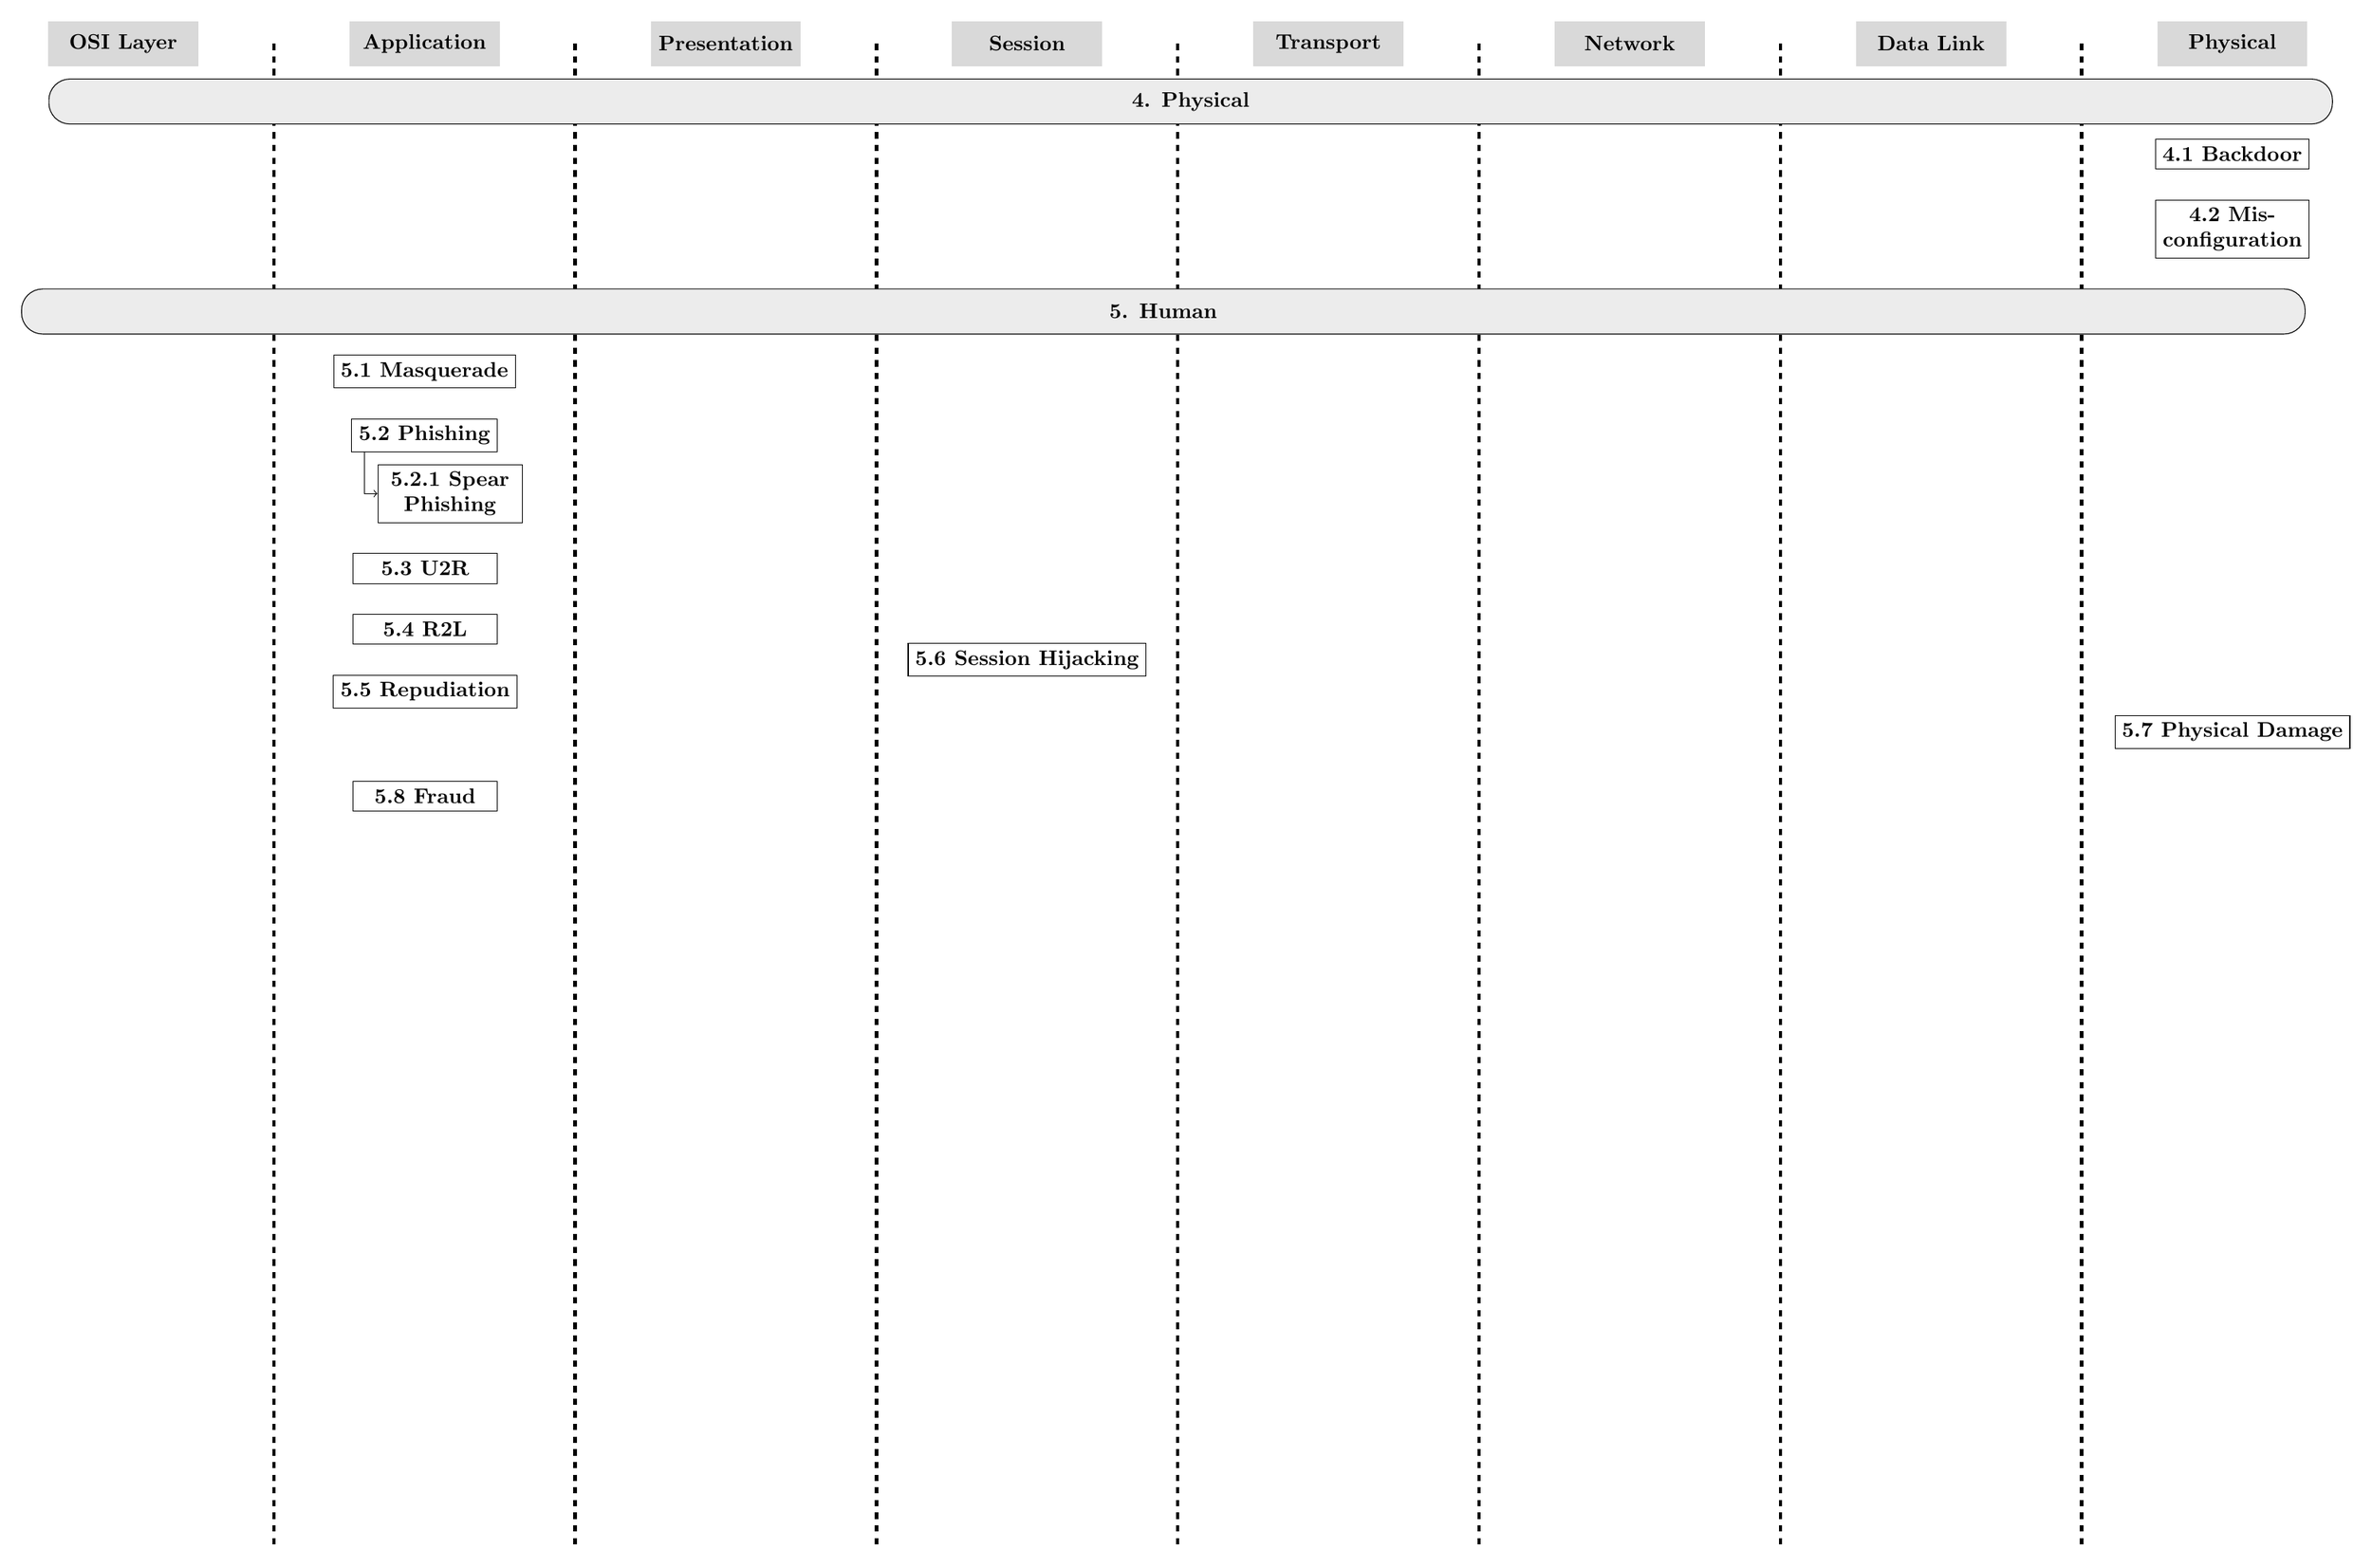
\begin{tikzpicture}
	
    \node [headerblock] (None) {OSI Layer};
\node [headerblock, right =\headerNodeDistance of None] (A) {Application};
\node [headerblock, right =\headerNodeDistance of A] (P) {Presentation};
\node [headerblock, right =\headerNodeDistance  of P] (S) {Session};
\node [headerblock, right =\headerNodeDistance  of S] (T) {Transport};
\node [headerblock, right =\headerNodeDistance  of T] (N) {Network};
\node [headerblock, right =\headerNodeDistance  of N] (D) {Data Link};
\node [headerblock, right =\headerNodeDistance  of D] (H) {Physical};
    \draw [dashed, ultra thick] ($(None.east)+(\halfHeaderNodeDistance,0)$) -- ($(None.east)+(\halfHeaderNodeDistance,-25)$);
\draw [dashed, ultra thick] ($(A.east)+(\halfHeaderNodeDistance,0)$) -- ($(A.east)+(\halfHeaderNodeDistance,-25)$);
\draw [dashed, ultra thick] ($(P.east)+(\halfHeaderNodeDistance ,0)$) -- ($(P.east)+(\halfHeaderNodeDistance ,-25)$);
\draw [dashed, ultra thick] ($(S.east)+(\halfHeaderNodeDistance ,0)$) -- ($(S.east)+(\halfHeaderNodeDistance ,-25)$);
\draw [dashed, ultra thick] ($(T.east)+(\halfHeaderNodeDistance ,0)$) -- ($(T.east)+(\halfHeaderNodeDistance,-25)$);
\draw [dashed, ultra thick] ($(N.east)+(\halfHeaderNodeDistance ,0)$) -- ($(N.east)+(\halfHeaderNodeDistance,-25)$);
\draw [dashed, ultra thick] ($(D.east)+(\halfHeaderNodeDistance ,0)$) -- ($(D.east)+(\halfHeaderNodeDistance,-25)$);

%%%%%%%%%%%%%%%%%%%%% Nodes %%%%%%%%%%%%%%%%%%%%%
	\node [sectionblock, below right =\smallY and -\headerNodeDistance of None] (S4) {4. Physical};
	
    \node [block, below = \largeY of H] (4_1) {4.1 Backdoor};
    \node [block, below = \medY of 4_1] (4_2) {4.2 Mis-\\configuration};
    
    \node [sectionblock, below left =\medY and -\headerNodeDistance of 4_2] (S5) {5. Human};

    \node [block, below =\largeY*4 of A] (5_1) {5.1 Masquerade};
    
	\node [block, below =\medY of 5_1] (5_2) {5.2 Phishing};
	\node [block, below right =\smallY and \shiftX of 5_2] (5_2_1) {5.2.1 Spear\\Phishing};
	
    \node [block, below left =\medY and \shiftX of 5_2_1] (5_3) {5.3 U2R};
	
    \node [block, below =\medY of 5_3] (5_4) {5.4 R2L};
	
	\node [block, below =\medY of 5_4] (5_5) {5.5 Repudiation};
   
	\node [block, below =\largeY*8 of S] (5_6) {5.6 Session Hijacking};
	
    \node [block, below =\largeY*9 of H] (5_7) {5.7 Physical Damage};

	\node [block, below =\largeY of 5_5] (5_8) {5.8 Fraud};

%%%%%%%%%%%%%%%%%%%%% Links %%%%%%%%%%%%%%%%%%%%%
	\draw[->] ($(5_2.south)-(\southXDisplacement, 0)$) |- (5_2_1.west);


\end{tikzpicture}
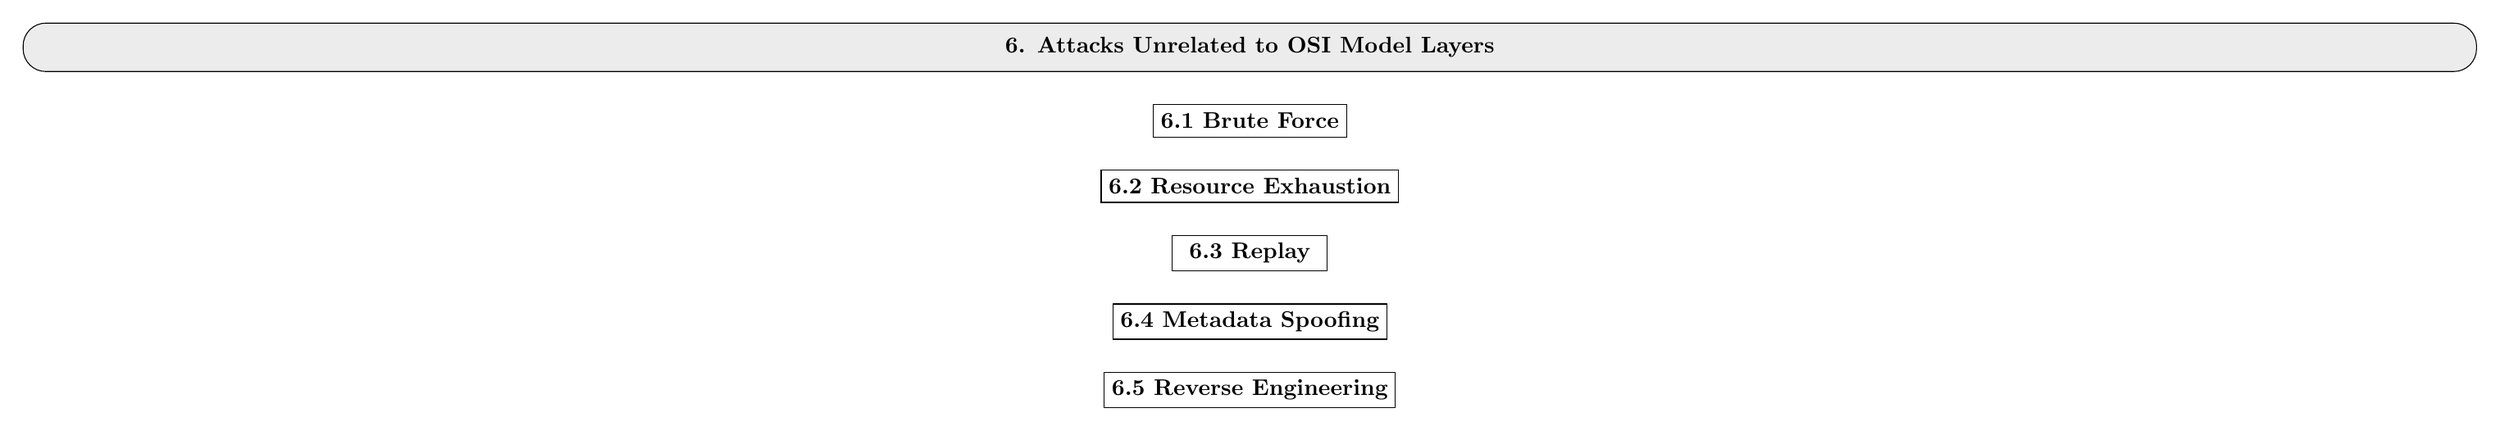
\begin{tikzpicture}

%%%%%%%%%%%%%%%%%%%%% Nodes %%%%%%%%%%%%%%%%%%%%%
	\node [sectionblock] (others) {6. Attacks Unrelated to OSI Model Layers};
    \node [block, below = \medY of others] (6_1) {6.1 Brute Force};
    \node [block, below = \medY of 6_1] (6_2) {6.2 Resource Exhaustion};
    \node [block, below = \medY of 6_2] (6_3) {6.3 Replay};
    \node [block, below = \medY of 6_3] (6_4) {6.4 Metadata Spoofing};
    \node [block, below = \medY of 6_4] (6_5) {6.5 Reverse Engineering};

\end{tikzpicture} 	
\end{document}
